\documentclass[main.tex]{subfiles}
\begin{document}

Suricata is a FOSS network threat detection engine capable of real time
intrusion detection and prevention and network security monitoring.
It can be configured based packet matching rules, and corresponding actions can
be triggered.

\begin{figure}[H]
  \centering
  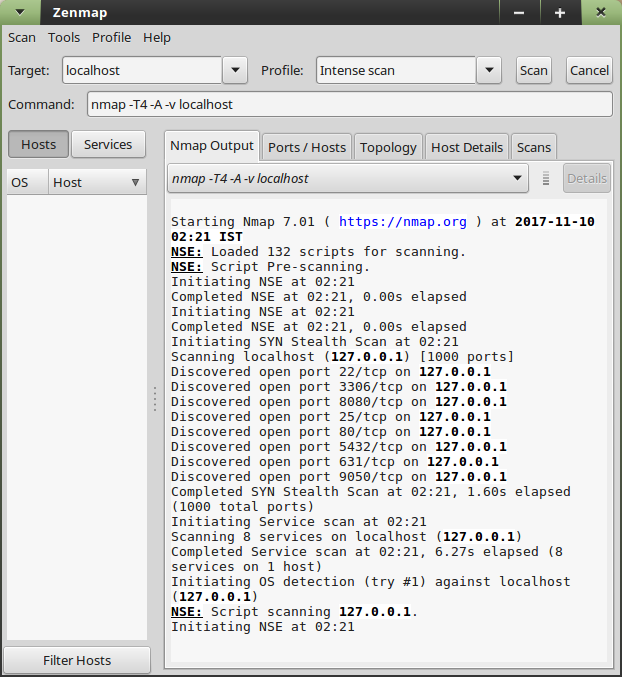
\includegraphics[width=\textwidth]{zenmap_scan.png}
  \caption{Zenmap scanning for open ports on the loopback interface}
\end{figure}

\begin{figure}[H]
  \centering
  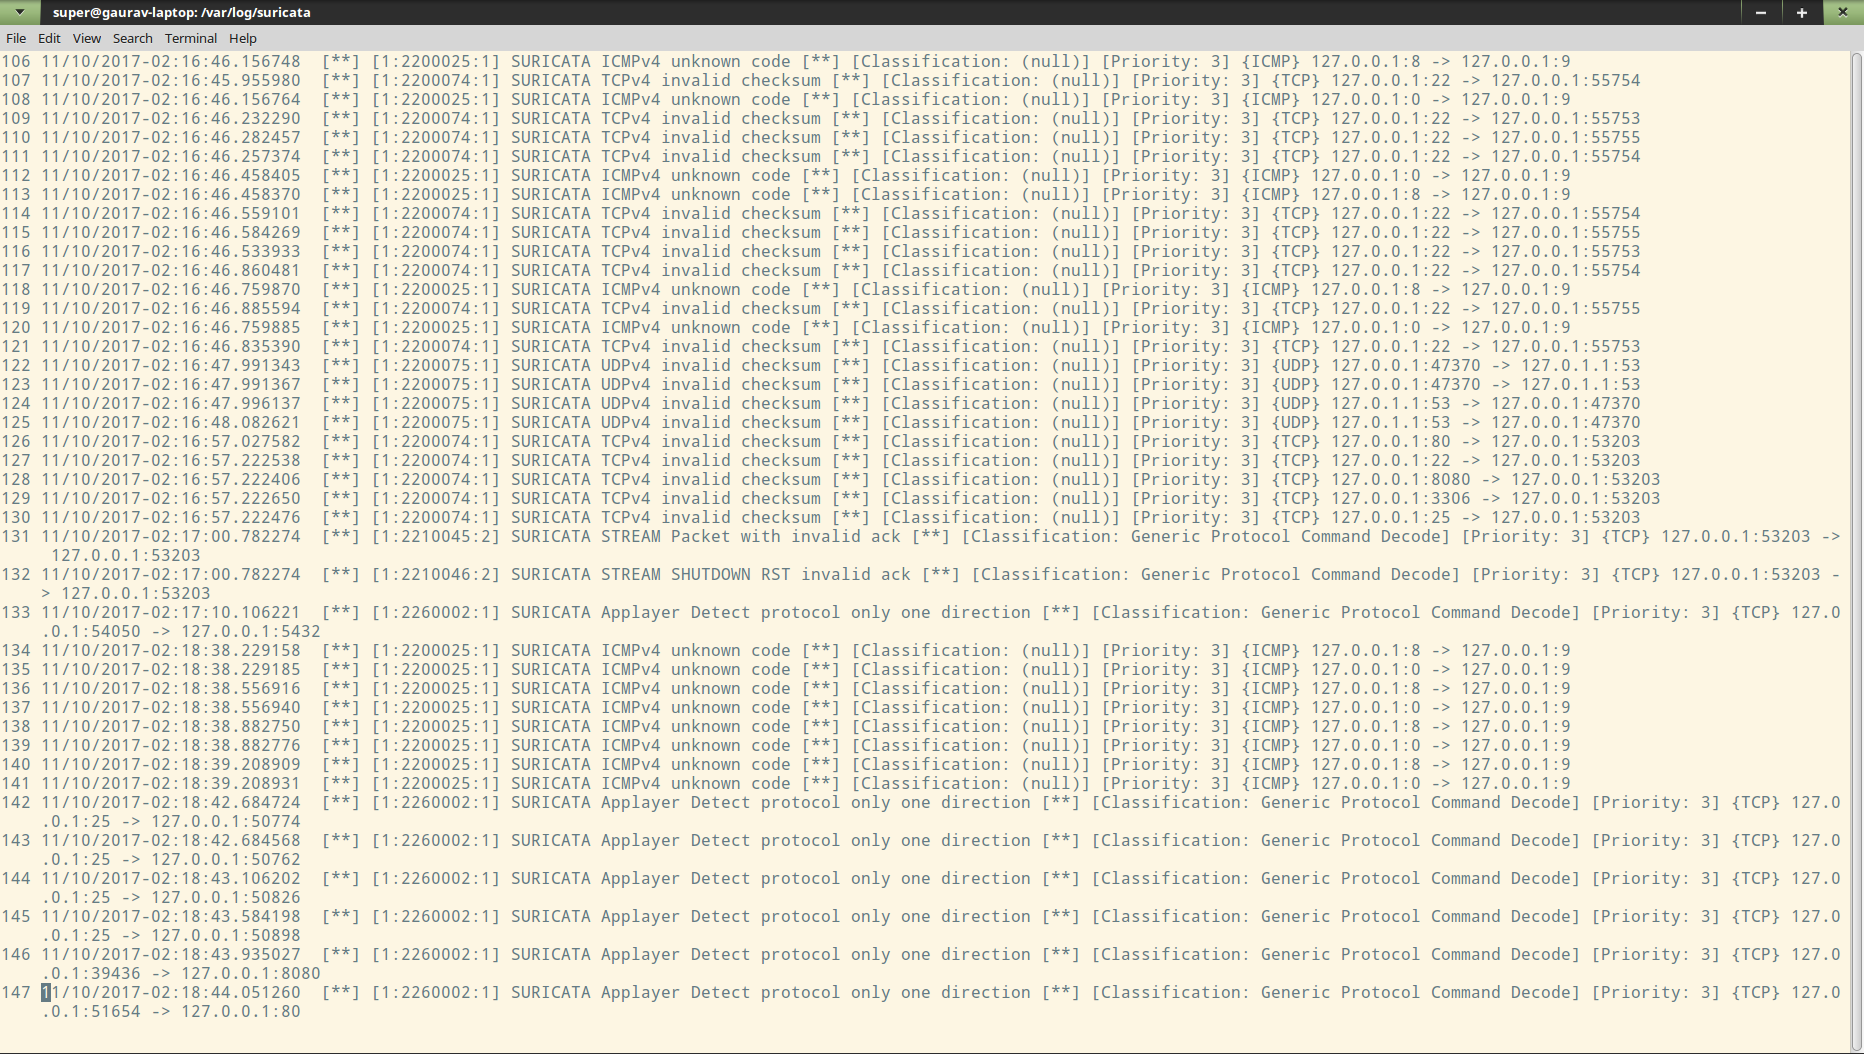
\includegraphics[width=\textwidth]{suricata_log.png}
  \caption{Suricata log using default Debain rules on loopback interface}
\end{figure}

Suricata inspects the network traffic using a powerful and extensive rules and
signature language, and has powerful Lua scripting support for detection of
complex threats.

Some of its main features are

\begin{itemize}
  \item Automatic protocol detection
  \item High performance multithreaded model
  \item TLS/SSL logging and analysis
  \item HTTP logging
  \item Variety of standard output formats
\end{itemize}

\end{document}
